\section{Experiments}

%\begin{figure}[!h]
%\centering
%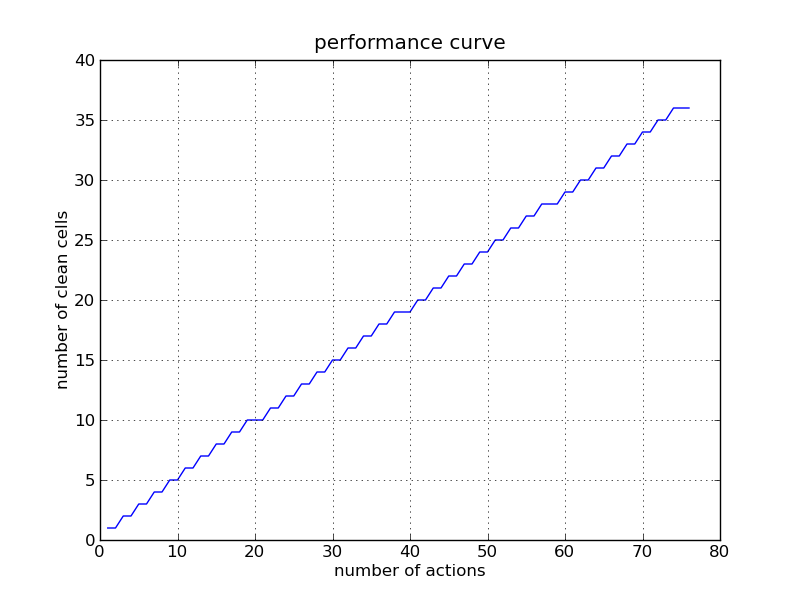
\includegraphics[scale=.35]{img/agent1.png}
%\caption{Performance of Memoryless Deterministic Agent}
%\label{fig:agent1}
%\end{figure}

%\begin{table}[h]
%    \centering
%    \begin{tabular}{|l|c|c|c|c|c|c|c|c|c|c|}
%        \hline
%        trials 1-10 & 495 & 625 & 514 & 647 & 842 & 614 & 550 & 532 & 532 & 924\\ \hline
%        trials 11-20 & 510 & 585 & 519 & 616 & 504 & 434 & 477 & 538 & 489 & 479\\ \hline
%        trials 21-30 & 385 & 562 & 531 & 591 & 551 & 458 & 515 & 711 & 662 & 439\\ \hline
%        trials 31-40 & 461 & 398 & 604 & 601 & 900 & 428 & 507 & 594 & 512 & 735\\ \hline
%        trials 41-50 & 572 & 574 & 490 & 498 & 578 & 517 & 380 & 444 & 605 & 506\\ \hline
%    \end{tabular}
%    \caption{Number of actions to take to clean $90\%$ of the room}\label{tab:agent2}
%\end{table}

%\begin{figure}[!h]
%        \centering
%        \subfloat[Number of actions]{
%                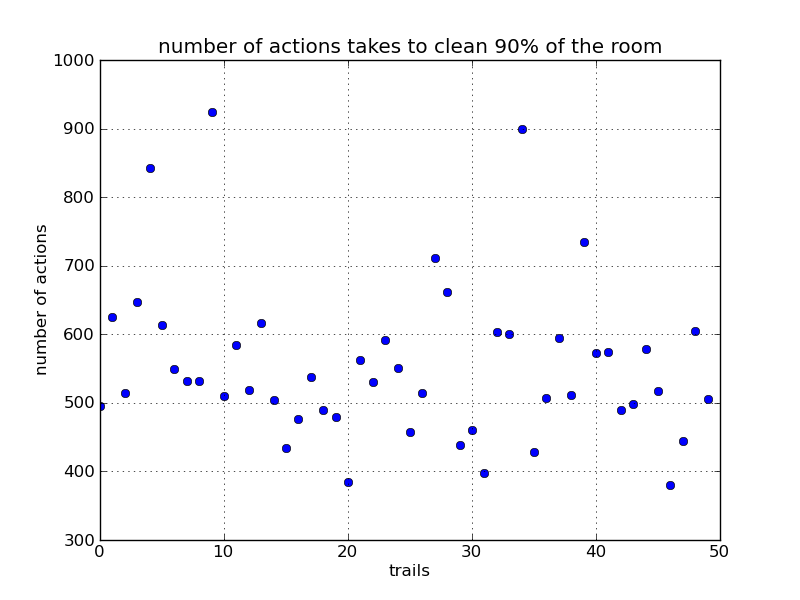
\includegraphics[scale=0.35]{img/num_actions.png}
%        }
%        \hspace{0.5in}
%        \subfloat[Performance curves]{
%                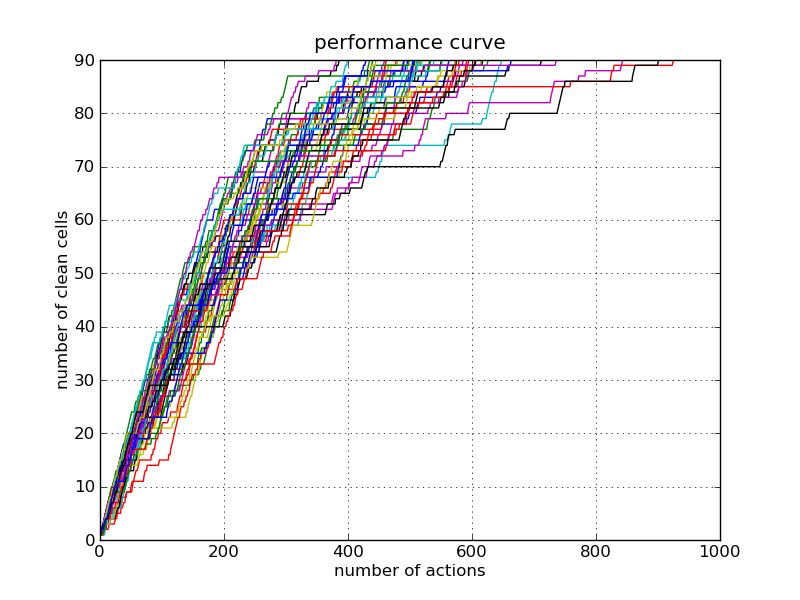
\includegraphics[scale=0.35]{img/rand.png}
%        }
%        \caption{Performance of randomized reflex agent}\label{fig:agent2}
%\end{figure}

